% Define document class
\documentclass[reprint,superscriptaddress,nobibnotes,amsmath,amssymb,aps,prx,hidelinks,linenumbers]{revtex4-2}

% Import relevant packages
\usepackage{showyourwork}
\usepackage{graphicx}
\usepackage{dcolumn}
\usepackage{bm}
\usepackage{multirow}
\usepackage[separate-uncertainty=true]{siunitx}
\usepackage{amsmath}
\usepackage[shortlabels]{enumitem}
\usepackage[page]{appendix}
\usepackage{xfrac}
\usepackage{printlen}
\usepackage[version=4]{mhchem}
\usepackage{blindtext}
% \usepackage[hidelinks]{hyperref}
\sisetup{
    list-units      = brackets,
    range-units     = brackets,
    range-phrase    = -,
    list-pair-separator= {, },
    list-separator  = {, },
    list-final-separator = {, }
    }
\renewcommand\appendixname{}
\newcommand{\papertitle}{Accurate Estimation of Diffusion Coefficients and their Uncertainties from Computer Simulation}
% \newcommand{\oMSD}{\ensuremath{\overline{\bm{s}^2}}}
% \newcommand{\oMSDs}[1]{\ensuremath{\overline{s^2}}(#1)}
% \newcommand{\oMSDi}{\ensuremath{\overline{s^2}_i}}
% \newcommand{\oMSDj}{\ensuremath{\overline{s^2}_j}}

\newcommand{\oMSD}{\ensuremath{\bm{x}}}
\newcommand{\oMSDs}[1]{\ensuremath{x}(#1)}
\newcommand{\oMSDi}{\ensuremath{x_i}}
\newcommand{\oMSDj}{\ensuremath{x_j}}
\newcommand{\oMSDn}{\ensuremath{x_n}}
\newcommand{\oMSDm}{\ensuremath{x_{n + m}}}
\newcommand{\moMSDn}{\ensuremath{\left<\oMSDn\right>}}
\newcommand{\moMSDm}{\ensuremath{\left<\oMSDm\right>}}
\newcommand{\modelmatrix}{\mathbf{A}}
\newcommand{\model}{\bm{m}}
\newcommand{\prob}[1]{\ensuremath{p(#1)}}
\newcommand{\probsq}[1]{\ensuremath{p[#1]}}
\newcommand{\nind}[1]{\ensuremath{N^\prime_{#1}}}
\newcommand{\code}[1]{#1}

\newcommand{\MSD}[1]{\big\langle\Delta\mathbf{r}{(#1)}^2\big\rangle}
\newcommand{\Dest}{\ensuremath{\widehat{D}^*}}
\newcommand{\D}{\ensuremath{D^*}}
\newcommand{\var}[1]{\ensuremath{\sigma^2[#1]}}
\newcommand{\varest}[1]{\ensuremath{\widehat{\sigma}^2[#1]}}
\DeclareMathOperator{\cov}{cov}
\DeclareMathOperator*{\argmax}{argmax}

\graphicspath{{figures/}}

% Redefine \maketitle so that it can be used twice (for supplementary)
\makeatletter
\def\maketitle{
\@author@finish
\title@column\titleblock@produce
\suppressfloats[t]}
\makeatother

% Begin!
\begin{document}

\let\oldaddcontentsline\addcontentsline% Store \addcontentsline
\renewcommand{\addcontentsline}[3]{}

% Title
\title{\papertitle}

% Author list
\author{Andrew R. McCluskey}
  \email{andrew.mccluskey@bristol.ac.uk}
  \affiliation{School of Chemistry, University of Bristol, Cantock's Close, Bristol, BS8 1TS, United Kingdom}
  \affiliation{European Spallation Source ERIC, Ole Maaløes vej 3, 2200 København N, DK}
\author{Samuel W. Coles}
  \affiliation{Department of Chemistry, University of Bath, Claverton Down, Bath, BA2 7AY, UK}
  \affiliation{The Faraday Institution, Quad One, Harwell Science and Innovation Campus, Didcot, OX11 0RA, UK}
\author{Benjamin J. Morgan}
  \email{b.j.morgan@bath.ac.uk}
  \affiliation{Department of Chemistry, University of Bath, Claverton Down, Bath, BA2 7AY, UK}
  \affiliation{The Faraday Institution, Quad One, Harwell Science and Innovation Campus, Didcot, OX11 0RA, UK}

% Abstract
\begin{abstract}
    Self-diffusion coefficients, $\D$, are routinely estimated from molecular dynamics simulations by fitting a linear model to the observed mean-squared displacements (MSDs) of mobile species.
    MSDs derived from simulation suffer from statistical noise, which introduces uncertainty in the resulting estimate of $\D$.
    An optimal scheme for estimating $\D$ will minimise this uncertainty, i.e., will have high statistical efficiency, and will give an accurate estimate of the uncertainty itself.
    We present a scheme for estimating $\D$ from a single simulation trajectory with high statistical efficiency and accurately estimating the uncertainty in the predicted value.
    The statistical distribution of MSDs observable from a given simulation is modelled as a multivariate normal distribution using an analytical covariance matrix for an equivalent system of freely diffusing particles, which we parameterise from the available simulation data. 
    We then perform Bayesian regression to sample the distribution of linear models that are compatible with this model multivariate normal distribution, to obtain a statistically efficient estimate of $D^*$ and an accurate estimate of the associated statistical uncertainty.
\end{abstract}

\maketitle 

\section{Introduction}

Mass transport is a fundamental physical process that is central to our understanding of fluids~\cite{sendner_interfacial_2009,shimizu_structural_2015,ghoufi_ultrafast_2016} and plays a critical role in biochemical systems~\cite{maccmmon_dynamics_1977,robertson_diffusion_2006}, and in solid-state devices such as batteries, fuel cells, and chemical sensors~\cite{eames_ionic_2015,morgan_understanding_2011,walsh_taking_2018}.
Molecular dynamics simulations are widely used to study microscopic transport processes, as they give direct insight into atomic-scale transport mechanisms and can be used to calculate macroscopic transport coefficients~\cite{morgan_relationships_2014,morgan_mechanistic_2021,poletayev_defect_2022,klepis_long_2009,wang_application_2011,zelovich_hydroxide_2019}.
These transport coefficients are formally defined in terms of ensemble averages.
Dynamical simulations, however, sample the full ensemble space stochastically, and parameters derived from simulation data are therefore only estimates of the true parameter of interest.
The statistical uncertainty associated with such estimates depends on the details of the simulation---e.g., size and timescale---and on the choice of estimation method.
An optimal estimation method will minimise the uncertainty in the computed quantity, i.e., it will have high statistical efficiency, and will also allow this uncertainty to be accurately estimated.

One commonly used parameter for quantifying atomic-scale mass transport is the self-diffusion coefficient, $\D$, which describes diffusion in the absence of a chemical potential gradient.
$\D$ is related to the ensemble-average mean squared displacement (MSD), $\MSD{t}$, via the Einstein relation~\cite{einstein_uber_1905,helfand_transport_1960},
%
\begin{equation}
    \D = \lim_{t\to\infty}\frac{\MSD{t}}{6t},
    \label{equ:einstein}
\end{equation}
%
where $t$ is elapsed time.
Because numerical simulations are finite in both time and space, MSDs obtained from simulation data always deviate from the true ensemble average MSD.
One can, however, compute an estimate of the self-diffusion coefficient, $\Dest$, by fitting a linear model to the observed MSD and using the gradient of this fitted model in place of $\MSD{t} / t$ in Eqn.~\ref{equ:einstein}.

The simplest approach to fitting a linear model to MSD data from simulation is ordinary least squares regression (OLS).
OLS gives analytical expressions for the ``best fit'' regression coefficients (the slope and intercept) and their respective uncertainties, making it easy to implement and quick to perform.
This procedure, however, is appropriate only for data that are both statistically independent and identically distributed.
Neither of these conditions hold for MSD data obtained from simulation, which instead are serially correlated and usually have unequal variances.
As a consequence, OLS is statistically inefficient, giving a relatively large statistical uncertainty in $\Dest$.
Furthermore, using the textbook OLS expression for the uncertainty in $\Dest$ significantly underestimates the true uncertainty in this estimate.
This underestimated uncertainty may cause overconfidence in the accuracy of values of $\D$ estimated using OLS, and using these data in downstream analyses may result in faulty inferences.
While the uncertainty associated with OLS estimates of $\D$ can, in principle, be accurately estimated by directly sampling over multiple repeated simulations, this approach greatly increases the total computational cost and therefore is often not practical.

\begin{figure*}
    \centering
    % \resizebox{\columnwidth}{!}{\includegraphics*{figure1.pdf}}
    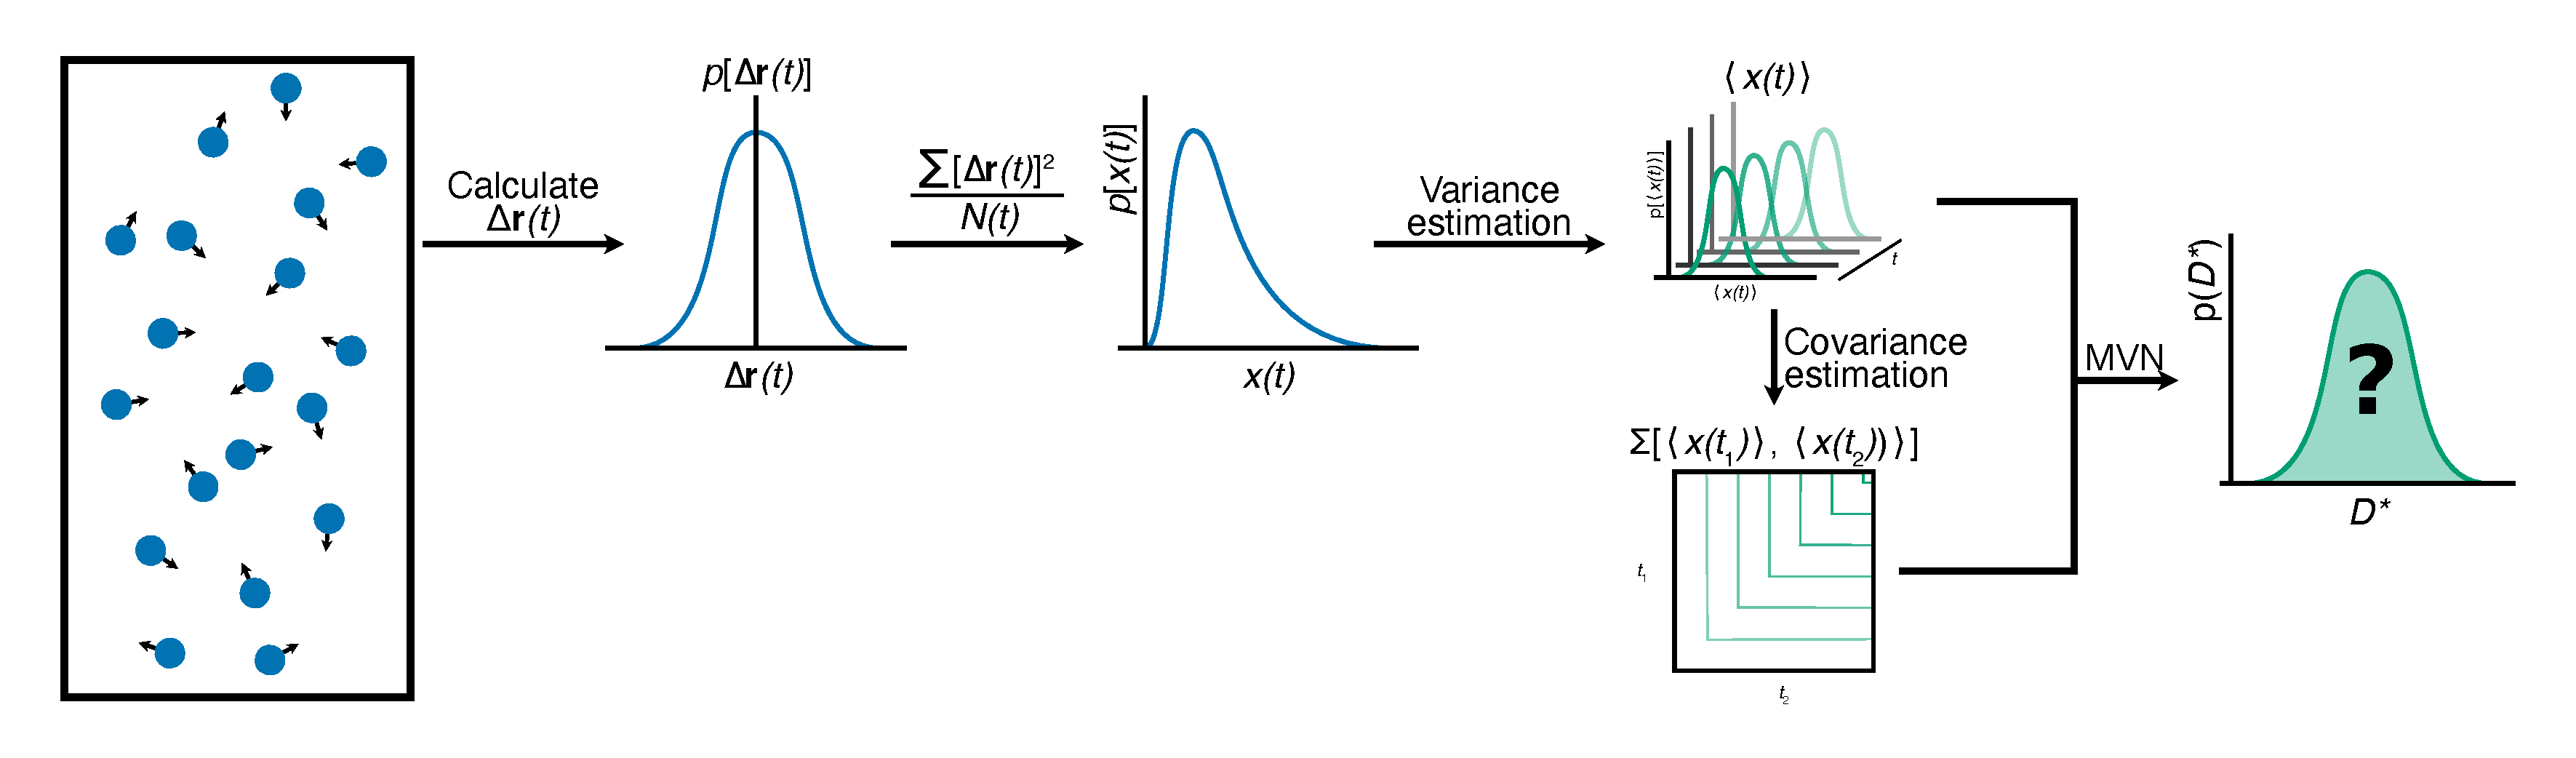
\includegraphics[width=\textwidth]{schematic.pdf}
    \caption{
        A schematic diagram of the Bayesian regression method described in this work, running from our simulations through the sampling of displacement, variance and covariance estimation and final the sampling process to give the marginal posterior distribution for $\D$.}
    \label{fig:schematic}
\end{figure*}

Here, we describe an approximate Bayesian regression method for estimating $\D$ with near-maximal statistical efficiency while also accurately estimating the corresponding statistical uncertainty, using data from a single simulation (Fig.~\ref{fig:schematic}).
We model the statistical population of simulation MSDs as a multivariate normal distribution, using an analytical covariance matrix derived for an equivalent system of freely diffusing particles, with this covariance matrix parameterised from the observed simulation data.
We then use Markov-chain Monte Carlo to sample the posterior distribution of linear models compatible with this multivariate normal model.
The resulting posterior distribution provides an efficient estimate for $\D$ and allows the associated statistical uncertainty in $\Dest$ to be accurately quantified.
This method is implemented in the open-source Python package \textsc{kinisi}~\cite{mccluskey_kinisi_2022}.

\section{Results}
\subsection{Background}

For a simulation of equivalent particles, the observed mean squared displacement as a function of time, $\oMSDs{t}$, can be computed as an average over equivalent particles and time origins:
%
\begin{equation}
  \oMSDs{t} = \frac{1}{N(t)}\sum^{N(t)}_{j=1}{\left[\Delta\mathbf{r}_j(t)\right]}^2,
  \label{equ:observed_msd}
\end{equation}
%
where $N(t)$ is the total number of observed squared-displacements at time $t$.
The resulting observed MSD is a vector, $\oMSD$, with individual elements $\oMSDi$.
Each element of this vector differs from the true ensemble-average MSD for that time by some unknown amount.
Fitting a linear model to $\oMSD$ gives an estimated self-diffusion coefficient, $\Dest$, which again differs from the true self-diffusion coefficient, $\D$, by some unknown amount.

Performing repeated simulations starting from different random seeds or with different histories will produce a set of replica trajectories, where each trajectory gives a different, statistically equivalent, observed MSD.
The set of all possible replica trajectories defines a population of hypothetical observed MSDs, and the MSD obtained from any one trajectory can be considered a random sample, $\bm{X}$, drawn from the multivariate probability distribution that describes this population, i.e, $\bm{X} \sim \prob{\oMSD}$.
Each potential MSD sample could, in principle, be fitted to a linear model to obtain a corresponding estimate for the self-diffusion coefficient; $\bm{X} \mapsto \Dest$.
The population of all such estimates therefore defines a probability distribution $\prob{\Dest}$.
The estimated diffusion coefficient obtained from a single simulation corresponds to a random sample drawn from this distribution, while the uncertainty in $\Dest$ is described by the shape of the full distribution $\prob{\Dest}$.

The statistical properties of $p(\Dest)$ depend on both the input MSD data and the choice of regression scheme used to obtain a ``best fit'' linear model.
An optimal estimation scheme for $\D$ should be unbiased, i.e., the expected value, $\mathbb{E}(\Dest)$, should equal the true self-diffusion coefficient $\D$, and should be maximally statistically efficient, i.e., the spread of $p(\Dest)$ around $\D$ should be minimised.
An estimation scheme should also provide an accurate estimate of the uncertainty in $\Dest$, to allow this estimated parameter to be used in subsequent inferential analysis.

For data that are both statistically independent and identically normally distributed, ordinary least squares regression (OLS) is unbiased and statistically efficient, and gives accurate estimates of the uncertainties in the resulting regression coefficients.
MSD data obtained from simulation, however, are neither statistically independent nor identically distributed.
The variances, $\var{\oMSDi}$, are correlated, since the displacement of each particle at time $t+\Delta t$ is necessarily similar to its displacement at time $t$, and hence, $\oMSDs{t}$ is similar to $\oMSDs{t+\Delta t}$.
These variances are also typically unequal---the data are heteroscedastic \cite{smith_random_1996,he_statistical_2018,UslerEtAl_JComputChem2023}. 
Because the key assumptions of the OLS method are not valid for MSD data, OLS gives statistically inefficient estimates of $\D$, while the estimated regression uncertainties obtained from the standard OLS statistical formulae significantly underestimate the true uncertainty in $\prob{\Dest_\mathrm{OLS}}$ (Fig.~\ref{fig:glswlsols}a).

\begin{figure}
    \centering
    % \resizebox{\columnwidth}{!}{\includegraphics*{figure1.pdf}}
    \includegraphics[width=\columnwidth]{glswlsols.pdf}
    \script{glswlsols.py}
    \caption{
        Example distributions of estimated self-diffusion coefficients, $\Dest$, calculated using (a) ordinary least squares (OLS), (b) weighted least squares (WLS), and (c) generalised least squares (GLS),
        from MSD data from \num{4096} individual simulations of \num{128} particles undergoing a \SI{128}{step} 3D lattice random walk, with a step size chosen so that the true diffusion coefficient $\D = 1$.
        In each panel, the grey curve shows the best-fit normal distribution for the simulation data, the upper horizontal bar shows the standard deviation of this distribution, and the lower horizontal bar shows the average estimated standard distribution given by the analytical expression for $\sigma[\prob{\Dest}]$ for each regression method.}
    \label{fig:glswlsols}
\end{figure}

Some improvement can be made by using weighted least squares (WLS) (Fig.~\ref{fig:glswlsols}b), where the residual for each observed MSD value is weighted by the reciprocal of its variance, $1/(\var{\oMSDi})$.
Like OLS, WLS is an unbiased estimator, and for heteroscedastic data it has higher statistical efficiency than OLS.
WLS still disregards correlations in $\oMSD$, however, and is therefore statistically inefficient, while the WLS estimated uncertainties for the regression coefficients still underestimate the true uncertainty in $\prob{\Dest_\mathrm{WLS}}$.

To optimally estimate the true ensemble-average MSD, and hence $\D$, from simulation data, it is necessary to account for both the changing variance and correlation structure of $\oMSD$.
Within the framework of linear regression, this can be achieved using generalised least squares (GLS).
GLS gives estimated regression coefficients, $\widehat{\beta}$, via
%
\begin{equation}
    \widehat{\beta} = \left(\modelmatrix^{\top}\mathbf{\Sigma}^{-1}\modelmatrix\right)^{-1}\modelmatrix^{\top}\mathbf{\Sigma}^{-1}\oMSD,
    \label{equ:gls}
\end{equation} 
%
where $\modelmatrix$ is the model matrix $\begin{bmatrix}\mathbf{1} & \bm{t}\end{bmatrix}$, with $\bm{t}$ the vector of observed times, and $\mathbf{\Sigma}$ is the covariance matrix for the observed MSD values.
For correlated heteroscedastic data, such as MSD data, GLS offers the theoretical maximum statistical efficiency---it achieves the Cram\'er--Rao bound~\cite{cramer_mathematical_1946,rao_information_1945,rao_selected_1994,darmois_sur_1945,aitken_on_1942}---and provides accurate analytical estimates of the uncertainty in the predicted regression coefficients (Fig.~\ref{fig:glswlsols}c).

An alternative method for estimating the ensemble-average MSD, and thus $\Dest$, from simulation data is Bayesian regression.
Like GLS, Bayesian regression can take into account both the changing variance and the correlation structure inherent in the data.
Rather than providing a singular ``best-fit'' estimate like GLS, Bayesian regression produces a posterior probability distribution for the regression coefficients.
The mean of this distribution serves as the point estimate of the coefficients and, in the absence of additional prior information, is equivalent to the GLS estimate, while the spread of the distribution quantifies the uncertainty in these estimates.
For data that is both heteroscedastic and correlated, such as MSD data from simulations, Bayesian regression, like GLS, is formally fully statistically efficient.

To estimate $\D$ from some observed MSD data, $\oMSD$, using Bayesian regression, we compute the posterior probability distribution $\prob{\model|\oMSD}$ for a linear model $\model = 6\D \bm{t} + c$, where $\D$ and $c$ are parameters to be estimated.
This posterior distribution is described by Bayes' theorem,
%
\begin{equation}
    \prob{\model|\oMSD} = \frac{\prob{{\oMSD|\model}}\prob{\model}}{\prob{\oMSD}},
    \label{equ:bayes}
\end{equation}
%
where $\prob{\oMSD|\model}$ is the probability of observing data $\oMSD$ given model $\model$, often described as the ``likelihood'', and $\prob{\oMSD}$ is the marginal probability of the observed data $\oMSD$.
Integrating over $\prob{\model|\oMSD}$ with respect to $c$ yields the marginal posterior distribution $\prob{\D|\oMSD}$, from which the best point-estimate $\Dest$ and distribution variance $\varest{\Dest}$ can be computed.

Given a sufficiently large number of observed squared displacements at each time $t$, the central limit theorem applies, and $\oMSD$ can be considered a sample from a multivariate normal distribution with log-likelihood
%
\begin{equation}
    \begin{aligned}{}
      \ln \prob{\oMSD|\model} = -\frac{1}{2}\big[ & \ln(\left|\mathbf{\Sigma}\right|) + {(\oMSD - \model)}^{\!\top}\mathbf{\Sigma}^{-1}(\oMSD - \model) \\ 
      & + k \ln(2\pi)\big],
    \end{aligned}
    \label{equ:loglike}
\end{equation}
%
where $\mathbf{\Sigma}$ is the observed MSD covariance matrix and $k$ is the length of the vector $\oMSD$, i.e., the number of time intervals for which we have observed MSD data.
Providing this likelihood function can be calculated, we can compute the posterior distribution $\prob{\model | \oMSD}$, which gives an optimally efficient point-estimate for $\D$ and a complete description of the associated uncertainty in $\Dest$.

\subsection{Approximating $\bm{\Sigma}$ from simulation data}

For Bayesian regression and GLS, we require the covariance matrix for the observed MSD, $\mathbf{\Sigma}$, which is generally unknown.
To proceed, we replace $\mathbf{\Sigma}$ with a model covariance matrix, $\mathbf{\Sigma^\prime}$, with a known analytical form, that we parameterise from the available simulation data.
Providing the correlation structure of $\mathbf{\Sigma^\prime}$ is similar to that of $\mathbf{\Sigma}$, this model correlation matrix can be used in approximate Bayesian or GLS schemes to estimate the ensemble-average MSD, and hence $\D$, with high efficiency and accurate estimated uncertainties.

We model the covariance matrix for the observed MSD from a given simulation using the covariance matrix for the MSD of an equivalent system of freely diffusing particles, $\mathbf{\Sigma^\prime}$.
For observed MSDs computed by averaging over numerically-independent sub-trajectories, the covariance matrix $\mathbf{\Sigma^\prime}$, in the long time limit, has elements (see SI)
%
\begin{equation}
  \Sigma^\prime\left[\oMSDi, \oMSDj\right]= \Sigma^\prime\left[\oMSDj, \oMSDi\right] =
  \var{\oMSDi} \frac{\nind{i}}{\nind{j}},\hspace{1em} \forall\,i \leq j,
  \label{equ:cvv}
\end{equation} 
%
where $\var{\oMSDi}$ are the time-dependent variances of the observed MSD, and $\nind{i}$ is the total number of numerically-independent observed squared-displacements for time-interval $i$, accounting for both overlapping sampling and concerted motion (see Eqn.~\ref{equ:der_var}).
We estimate the variances $\var{\oMSDi}$ using the standard result that the variance of the mean of a sample scales inversely with the number of independent constituent observations.
Specifically, we approximate the variance $\varest{\oMSDi}$ (see SI) by rescaling the observed variance of the squared displacement for time interval $i$ by the number of numerically-independent contributing sub-trajectories, $\nind{i}$;
%
\begin{equation}
  \varest{\oMSDi} \approx \frac{1}{\nind{i}}\var{\Delta r_i^2}.
  \label{equ:varestMSD}
\end{equation}
%

Rescaling by the number of numerically-independent contributing sub-trajectories has the effect of renormalising the variance of the observed squared displacements to account for correlations between particle squared displacements computed from overlapping time windows. 
An alternative approach to renormalising $\var{x_i}$ is to use a non-parametric block-averaging procedure~\cite{flyvbjerg_error_1989,frenkel_understanding_2023,materzanini_high_2021}, which gives undesirable results for a random walk (see SI). 
The block-averaging approach, additionally, requires numerical convergence with respect to block size, which is not guaranteed for time windows with few independent observations. 
We require $\var{x_i}$ at all observed time intervals, $i$, making block averaging on large data sets computationally prohibitive. 

The estimated variance $\varest{\oMSD}$ can be calculated from a single simulation trajectory, and provides an accurate estimate of the true variance $\var{\oMSD}$.
To demonstrate this, we performed \num{4096} independent simulations of \num{128} particles undergoing a three-dimensional cubic-lattice random walk of \num{128} steps per particle.
Using data from all \num{4096} simulations, we first compute the true simulation MSD and its variance (Fig.~\ref{fig:msd}a).
We also compute the MSD and estimated variance using data from a single simulation trajectory (Fig.~\ref{fig:msd}b), using the scheme described above.
A quantitative comparison between the true MSD variance and the single-trajectory estimated MSD variance is made in Fig.~\ref{fig:msd}c: the close numerical agreement confirms that Eqn~\ref{equ:varestMSD} can be used to estimate $\var{\oMSD}$, which can then be used to parameterise the model covariance matrix $\mathbf{\Sigma^\prime}$ via Eqn.~\ref{equ:cvv}.

\begin{figure}
    \centering
    % \resizebox{\columnwidth}{!}{\includegraphics*{figure2.pdf}}
    \includegraphics[width=\columnwidth]{msd.pdf}
    \script{msd.py}
    \caption{
        Comparison of the numerical variance in observed MSD from multiple replica simulations and the estimated variance in observed MSD given by rescaling the variance in observed squared displacements (Eqn.~\ref{equ:varestMSD}).
        Panel (a) shows the mean observed MSD from \num{4096} simulations of \num{128} particles undergoing a 3D lattice random walk of \num{128} steps per particle, with error bars of $\pm2\sigma[\oMSDi]$.
        Panel (b) shows the MSD from just one simulation, with error bars of $\pm2\widehat{\sigma}[\oMSDi]$, obtained via Eqn.~\ref{equ:varestMSD}.
        Panel (c) plots the numerical variance against the estimated variance from a single simulation as a function of timestep $i$.
        %Raw simulation data~\cite{mccluskey_zenodo_2022} and scripts~\cite{mccluskey_github_2022} to generate this figure are available under CC BY 4.0/MIT licences.
    }
    \label{fig:msd}
\end{figure}


The practical implementation of both GLS and Bayesian regression requires that the covariance matrix $\mathbf{\Sigma^\prime}$ is invertible (positive definite); see Eqns.~\ref{equ:gls} and \ref{equ:loglike}.
The estimated MSD variances derived from simulation data via Eqn.~\ref{equ:varestMSD} are statistically noisy and using these to directly parameterise $\mathbf{\Sigma^\prime}$ can yield non-invertible singular matrices.
To make our scheme numerically tractable, we therefore fit our estimated MSD variances to the analytical variance for an analogous system of particles undergoing random walks~\cite{smith_random_1996};
%
\begin{equation}
    \var{\oMSDi} = a\frac{t^2_i}{\nind{i}},
    \label{equ:variance}
\end{equation}
%
where $a$ is a scaling parameter determined by fitting Eqn.~\ref{equ:variance} to the directly estimated MSD variances.
This smoothing of $\var{\oMSDi}$ guarantees that the resulting model covariance matrix $\mathbf{\Sigma^\prime}$ is invertible and thus suitable for GLS or Bayesian regression.

To illustrate the complete numerical procedure for deriving the model covariance matrix, $\bm{\Sigma^\prime}$, we present in Fig.~\ref{fig:covariances} the MSD covariance matrix for \num{4096} random-walk simulations, as described above, at three differing levels of approximation:
the numerically converged covariance matrix, $\bm{\Sigma}$, computed using the data from all \num{4096} simulations (Fig.~\ref{fig:covariances}a);
the corresponding analytical model covariance matrix, $\mathbf{\Sigma^\prime}$, defined by Eqn.~\ref{equ:cvv} and parametrised using analytical variances $\var{\oMSDi}$ (Fig.~\ref{fig:covariances}b); and the average model covariance matrix obtained by parametrising Eqn.~\ref{equ:cvv} using smoothed variances estimated from individual simulation trajectories, and averaging over the resulting set of all \num{4096} matrices (Fig.~\ref{fig:covariances}c).

\begin{figure}
    \centering
    % \resizebox{\columnwidth}{!}{\includegraphics*{figure3.pdf}}
    \includegraphics[width=\columnwidth]{covariances.pdf}
    \script{covariances.py}
    \caption{
        (a) The numerical MSD covariance matrix $\bm{\Sigma}$ calculated using MSD data from \num{4096} simulations of \num{128} particles undergoing a 3D lattice random walk of \num{128} steps per particle.
        (b) The analytical MSD covariance matrix $\bm{\Sigma^\prime}$ (Eqn.~\ref{equ:cvv}), parametrised using analytical random-walk variances $\var{\oMSDi}$.
        (c) The MSD covariance matrix obtained applying the numerical scheme described in the main text to each individual random walk simulation, averaged over all \num{4096} such simulations.
        Colour bars in (a--c) show the covariance, $\Sigma\left[\oMSDi, \oMSDj\right]$.
        The off-diagonal panels show difference plots, computed as per-element ratios between pairs of covariance matrices (a--c).
        %Raw simulation data~\cite{mccluskey_zenodo_2022} and scripts~\cite{mccluskey_github_2022} to generate this figure are available under CC BY 4.0/MIT licences.
    }
    \label{fig:covariances}
\end{figure}


While the analytical and average estimated covariance matrices show some systematic deviation from the numerically converged covariance matrix, the general correlation structure is preserved.
The discrepancy between the model and numerical covariance matrices largely stems from the approximation made in deriving the analytical form that $t$ is large, which leads to an overestimation of the variance at low $t$.
Despite this, the average estimated covariance matrix reproduces well the correlation structure of the true numerical covariance matrix, indicating that the covariance matrices estimated from individual simulation trajectories may be used within approximate GLS or Bayesian regression schemes to estimate $\D$ and $\var{\Dest}$.

\subsection{Validation}

\begin{figure*}[ht!]
    \centering
    % \resizebox{\textwidth}{!}{\includegraphics*{figure4.pdf}}
    \includegraphics[width=\textwidth]{random_walk.pdf}
    \script{random_walk.py}
    \caption{
        (a) Observed MSD from a single simulation of 128 particles undergoing a 3D-lattice random walk of 128 steps per particle (dark line).
        The green shading shows the corresponding posterior distribution $\prob{\model|\oMSD}$ of linear models compatible with the observed MSD data $\oMSD$, calculated using the scheme described in the main text.
        The variegated shading indicates compatibility intervals of \SIlist[list-final-separator = {, and }]{1;2;3}{\sigma}$[\prob{\model|\oMSD}]$.
        (b) The marginal posterior distribution $\prob{\Dest|\oMSD}$ obtained from the posterior distribution of linear models in (a).
        The mean of this distribution gives the point estimate $\Dest$ for this simulation input data.
        The blue horizontal bar shows an interval of one standard deviation in $\prob{\Dest|\oMSD}$.
        (c) Probability distribution of point-estimates $\prob{\Dest}$ obtained from \num{4096} individual random-walk simulations.
        Each simulation has been analysed as in (a) and (b) to yield a single corresponding point estimate $\Dest$.
        The grey line shows the distribution of point estimates, $\prob{\Dest_\mathrm{num}}$, obtained using Bayesian regression with a mean vector and numerical covariance matrix derived from the complete dataset of all \num{4096} simulations.
        The pink horizontal bar shows an interval of one standard deviation in $\prob{\Dest}$.
        (d) Probability distribution of estimated variances, $\varest{\Dest}$, for individual random-walk simulations, compared to the true sample variance (pink vertical line) $\var{\Dest}$.
    } 
    \label{fig:random_walk}
\end{figure*}

To demonstrate the complete approximate Bayesian regression scheme, as described above, we present two distinct examples.
First, we consider a simple 3D-lattice random walk, where the true self-diffusion coefficient $\D$ is specified by the simulation parameters, and a well-converged numerical covariance matrix can be obtained with relatively low computational cost, which allows us to directly compare the estimates produced by our method to ``best case'' estimates from a hypothetical method with access to the true covariance matrix.
Second, we consider an example real-world system---the lithium-ion solid electrolyte \ce{Li7La3Zr2O12} (LLZO)---which represents an application of our method to a well-studied material of practical interest for solid-state lithium-ion batteries \cite{MuruganEtAl_AngewChemIntEd2007,burbano_sparse_2016,morgan_lattice_2017,SquiresEtAl_PhysRevMater2022}.

Fig.~\ref{fig:random_walk}a shows the observed MSD from a single 3D-lattice random-walk simulation, along with the estimated posterior distribution of linear models compatible with the observed MSD data, $\prob{\model|\oMSD}$, calculated via Eqns.~\ref{equ:bayes} and \ref{equ:loglike}.
The corresponding marginal posterior distribution of estimated diffusion coefficients $\prob{\D|\oMSD}$ is shown in Fig.~\ref{fig:random_walk}b; this distribution is approximately Gaussian and is centred on the true self-diffusion coefficient $\D = \num{1}$, demonstrating that for this example trajectory we obtain a good point-estimate of $\D$.

To evaluate the overall performance of our method, we repeat our analysis on the full set of \num{4096} random-walk simulations.
Fig.~\ref{fig:random_walk}c presents a histogram of the resulting point estimates of $\D$, with each estimate derived as the mean of the posterior distribution $\prob{\D|\oMSD}$ using input data from an individual simulation.
We also show the probability distribution of estimated diffusion coefficients obtained using Bayesian regression with a mean vector and covariance matrix derived numerically from all \num{4096} simulations (solid line).
This latter distribution represents the distribution of ``best possible'' estimates of $\D$ and exhibits the minimum possible theoretical variance.
The close agreement between these two distributions demonstrates that our approximate Bayesian regression scheme yields nearly optimal estimates of $\D$ using data from individual simulations.
The distribution of estimated diffusion coefficients from single simulations is slightly broader than the exact numerical results.
This minor deviation is a consequence of the overestimation of $\varest{\oMSDi}$ at short times, noted above, which results from our use of the long-time limit in the derivation of the analytical model covariance matrix.

We next consider the degree to which our method can quantify the uncertainty in $\Dest$ when using input data from a single simulation.
Fig.~\ref{fig:random_walk}d shows the distribution of estimated variances $\varest{\Dest}$, with each sample calculated from an individual simulation trajectory.
We also show the true variance of individual point estimates, $\var{\Dest}$, which characterises the spread of the histogram in Fig.~\ref{fig:random_walk}c.
The distribution of estimated variances is biased relative to the true variance and skewed, due to numerical differences between the true covariance matrix $\mathbf{\Sigma}$ and the model covariance matrix $\mathbf{\Sigma^\prime}$ (further details are provided in the SI).
In general, however, the distribution of the estimated variance shows good agreement with the true sample variance.
Notably, the precision of this estimate is significantly greater than obtained using OLS or WLS and their corresponding textbook statistical formulae.

We next benchmark our method using data from simulations of the cubic lithium-ion solid electrolyte \ce{Li7La3Zr2O12} (c-LLZO).
We performed a single simulation of \num{1536} atoms (\num{448} Li ions) at \SI{700}{K} for \SI{6}{\nano\second} (full simulation details are provided in the Methods section).
To generate multiple statistically equivalent trajectories, the resulting simulation data was partitioned into \num{480} effective trajectories, each approximately $\sim\SI{100}{\ps}$ in length, and containing data for \num{56} lithium ions.
We then perform the same approximate Bayesian regression analysis as above on each effective trajectory, excluding the first \SI{10}{ps} of MSD data in each case to remove short-time data corresponding to ballistic and sub-diffusive regimes \cite{he_statistical_2018}.

The resulting distribution of the point estimates, $\Dest$, from analysis of all \num{512} effective trajectories is shown in Fig.~\ref{fig:diffusion}a.
Again, the corresponding distribution of $\Dest$ estimates derived using Bayesian regression and a well-converged numerical covariance matrix calculated from the full LLZO dataset is also shown for comparison.
The distribution $\prob{\Dest}$ obtained using the model covariance matrix and parametrised separately for each individual effective simulation is highly similar to that obtained using the aggregate numerical covariance matrix calculated from the complete simulation dataset.
This close agreement mirrors the results for our random walk simulations (see the SI for a similar comparison of the OLS, WLS, and GLS as shown in Fig.~\ref{fig:glswlsols}), and confirms that our method yields accurate and statistically efficient estimates for $\D$, even for real-world simulation data.

\begin{figure}[tb]
    \centering
    % \resizebox{\columnwidth}{!}{\includegraphics*{figure5.pdf}}
    \includegraphics[width=\columnwidth]{diffusion.pdf}
    \script{diffusion.py}
    \caption{
      (a) Probability distribution of point estimates $\prob{\Dest}$ for \num{512} effective simulations of LLZO (orange histogram).
      The grey line shows the distribution $\prob{\Dest_\mathrm{num}}$ obtained using Bayesian regression with the complete LLZO dataset as input.
      The pink bar shows an interval of one standard deviation $\sigma[\prob{\Dest}]$.
      (b) Probability distribution of estimated variances, $\varest{\Dest}$, for individual LLZO effective simulations, compared to the true sample variance (pink vertical line) $\var{\Dest}$.
      %Raw simulation data~\cite{mccluskey_zenodo_2022} and scripts~\cite{mccluskey_github_2022} to generate this figure are available under CC BY 4.0/MIT licences. 
    }
    \label{fig:diffusion}
\end{figure}

We also consider the probability distribution of estimates of the variance in $\Dest$ calculated for each effective trajectory (Fig.~\ref{fig:diffusion}b), which we compare to the true variance in $\Dest$ for our method; i.e., the variance of the histogram in Fig.~\ref{fig:diffusion}a.
While the estimated variances deviate somewhat from the true distribution $\prob{\var{\Dest}}$, the agreement is reasonable and mirrors our results for the random walk simulations.
Hence, our method provides reasonably accurate estimates of the uncertainty in $\Dest$ for our c-LLZO dataset, even when applied to single effective trajectories with limited displacement data (only 56 mobile ions, and \SI{25}{ps} simulation length).

\subsection{$\var{\Dest}$ scaling and comparison to OLS, WLS, and GLS}

\begin{figure}[htb]
    \centering
    % \resizebox{\columnwidth}{!}{\includegraphics*{figure6.pdf}}
    \includegraphics[width=\columnwidth]{stat_eff.pdf}
    \script{stat_eff.py}
    \caption{
      Scaling of $\var{\Dest}$ with simulation size for OLS (pink), WLS (blue), our approximate Bayesian regression method (green), and GLS (orange).
      (a) Scaling versus number of mobile particles, $N_\mathrm{atoms}$.
      (b) Scaling versus total simulation time, $t_\mathrm{max}$.
      Solid lines show fitted power law relationships for each dataset.
      The WLS and GLS data are obtained using numerically determined variances and covariance, respectively, from a set of \num{512} repeat simulations for each combination of $N_\mathrm{atoms}$ and $t_\mathrm{max}$.
    }
    \label{fig:stat_eff}
\end{figure}

Fig.~\ref{fig:stat_eff} presents an analysis of the variation in $\var{\Dest}$ as the number of mobile particles (Fig.~\ref{fig:stat_eff}a) and the total simulation time (number of steps) (Fig.~\ref{fig:stat_eff}b) are changed.
We compare four methods for estimating $\D$ from the observed MSD data: OLS, WLS, the approximate Bayesian regression method described here, and GLS.
When estimating $\D$ using WLS and GLS, we calculate the variances and the covariance matrix, respectively, numerically, using the complete set of \num{512} simulations.
Each data point in Fig.~\ref{fig:stat_eff} represents the variance across point-estimates of $\D$ derived from \num{512} individual 3D-lattice random walk simulations, for each combination of $N_\mathrm{atoms}$ and $t_\mathrm{max}$.
The GLS dataset corresponds to an optimally efficient estimator for linear regression of observed MSD data, equivalent to performing Bayesian regression with the numerical covariance matrix and an uninformative prior.

Our approximate Bayesian regression method performs similarly to GLS, with a numerically converged covariance matrix, and gives significantly reduced uncertainty in $\Dest$ compared to OLS or WLS, for all simulation sizes and lengths considered.
Moreover, our method scales better than OLS or WLS as the total simulation time is increased.
The approximate Bayesian regression method in this manuscript therefore presents a significant improvement over more conventional methods such as OLS and WLS, by enabling more precise estimates of $\D$ across varied simulation sizes at equivalent computational cost.

\section{Summary and Discussion}

We have introduced and evaluated an approximate Bayesian regression method for estimating the self-diffusion coefficient, $\D$, from molecular dynamics simulation data.
We consider the observed mean-squared displacement data from a single simulation as a random sample, $\bm{X}$, from a population of potential MSDs generated by equivalent replica simulations, $\bm{X}\sim p(\oMSD)$.
We model this population using a multivariate normal distribution, $p(\oMSD) = \mathcal{N}(\model, \mathbf{\Sigma})$, with mean vector $\model = 6\D\bm{t} + c$, where $\D$ and $c$ are model parameters to be determined.

To model the covariance matrix, we use an analytical solution derived for an equivalent system of freely diffusing particles.
To parameterise this model covariance matrix, we rescale the variance of the observed squared displacements from the input simulation trajectory, followed by a smoothing step to ensure a positive-definite matrix.
The resulting model covariance matrix preserves the correlation structure of the true simulation MSD covariance matrix, and gives a multivariate normal model for the population of observable simulation MSDs that depends solely on the model parameters, $\D$ and $c$.

We use Markov-Chain Monte Carlo to sample the posterior distribution of linear models compatible with the observed MSD data.
This approach yields a marginal posterior distribution, $\prob{\D | \oMSD}$, that gives a statistically efficient point estimate for $\D$ and allows the associated statistical uncertainty, $\var{\Dest}$, to be quantified.

We have benchmarked our approach using simulation data for an ideal 3D lattice random walk and for the lithium-ion solid electrolyte \ce{Li7La3Zr2O12} (LLZO).
In both cases, we obtain a distribution of estimates for $\D$ that closely matches the theoretically optimal distribution obtained using a numerical covariance matrix derived from a large number of replica simulation trajectories.

We obtain estimates for $\D$ that are unbiased, with near-optimal statistical efficiency, using input data from single simulation trajectories.
The approximate Bayesian regression scheme therefore provides more accurate single-point estimates of the self-diffusion coefficient than the commonly used OLS or WLS methods, when applied to the same input simulation data.
The improved statistical efficiency of this method, when compared to OLS or WLS, enables the estimation of $\D$ with equivalent accuracy from considerably smaller simulations---either in terms of timescale or system size. 
This reduces the overall computational cost when compared to studies that use OLS or WLS for estimating a linear fit to simulation MSD data.
Alternatively, this approach provides the possibility to estimate $\D$ with greater precision, given simulation trajectories of equal size.

Our method also provides reasonable estimates of the statistical uncertainty in the estimated value $\Dest$, in contrast to OLS and WLS which systematically significantly underestimate the uncertainty in regression coefficients when applied to simulated MSD data. 
While these estimated statistical uncertainties can still differ from the true (but unknown) uncertainty in $\Dest$, particularly when using short-timescale simulation data, they allow for scientifically meaningful comparisons to be made between estimated diffusion coefficients across different materials or under varying conditions, such as changes in temperature, or between computational findings and experimental results.
Furthermore, these uncertainties allow for quantitative downstream analysis, such as the application of Arrhenius (on non-Arrhenius) type models to describe the temperature dependence of self-diffusion.

The approximate Bayesian regression scheme presented here provides a statistically efficient means of estimating the self-diffusion coefficient, $\D$, from molecular dynamics simulation data.
It improves upon textbook approaches by providing accurate point estimates of $\D$ with near-optimal statistical efficiency, while also providing a reasonable description of the uncertainty in these estimates.
The high statistical efficiency of our method allows for the use of smaller simulations, which can significantly reduce computational costs.
Overall, our method offers significant advantages over more conventional methods of estimating self-diffusion coefficients from atomistic simulations.
We have implemented this procedure in the open-source package \textsc{kinisi} \cite{mccluskey_kinisi_2022}, which we hope will support its use within the broader simulation community across a range of materials science contexts.

\section{Methods}

\subsection{Numerical implementation in KINISI}
\label{sec:implementation}
We have implemented the approximate Bayesian estimation method described in the main text in the open-source Python package \textsc{kinisi}~\cite{mccluskey_kinisi_2022}, under the MIT licence. 

\textsc{kinisi} uses overlapping sliding window sampling when calculating the observed mean squared displacement at each time interval $t$ (see Eqn.~\ref{equ:observed_msd}).
For a given time interval, $t$, the maximum number of observations is $N_{\mathrm{atoms}} \times (N_{t} - i)$ displacements, where $N_{\mathrm{atoms}}$ is the number of atoms, $N_{t}$ is the total number of timesteps, and $i$ is the index of the timestep (where \num{1} is the index for the shortest timestep).
To estimate the variance of the observed MSD, we rescale the variance of observed squared displacements by the number of numerically-independent sub-trajectories in the simulation, $\nind{i} = N_{\mathrm{atoms}} \times N_{t} / i$, as presented in Eqn.~\ref{equ:varestMSD}.  

The parametrisation of the covariance matrix from the variances $\var{\oMSDi}$ and the number of independent observations $\nind{i}$ is defined by Eqn.~\ref{equ:cvv}. 
The covariance matrix is only constructed for values of $t$ where the particle motion is considered to be in the long-time diffusive limit, with this threshold set by the user to a value appropriate for their system and simulation data. 
For the examples presented in the main manuscript, we consider particles to be in the diffusive regime from $t=\num{4}$ for the random walk trajectories and from $t=\SI{10}{\pico\second}$ for the LLZO simulations.

\textsc{kinisi} uses ordinary least squares to obtain an initial guess for the gradient and intercept of the linear model describing the observed MSD.
This initial guess is then used as the starting point for minimising the negative maximum a posteriori (the peak of the posterior distribution as per Eqn.~\ref{equ:bayes}), with the improper prior that $\D \ge 0$~\cite{broyden_convergence_1970,fletcher_new_1970,goldfarb_family_1970,shanno_conditioning_1970}.
The log-likelihood calculation (Eqn.~\ref{equ:loglike}) uses the Moore-Penrose generalisation of the inverse of a Hermitian matrix~\cite{moore_on_1920,bjerhammar_application_1951,penrose_generlized_1955}. 

To sample the joint posterior probability distribution of the linear model, \textsc{kinisi} uses the \textsc{emcee} package~\cite{foremanmackey_emcee_2019}, which implements Goodman and Weare's affine invariant Markov chain Monte Carlo ensemble sampler~\cite{goodman_ensemble_2010}. 
When sampling $\prob{\D|\model}$ we again apply the improper prior $\D \ge 0$.
The sampling process uses \num{32} walkers for \num{1500} steps, with the first \num{500} steps discarded as a burn-in period.
The sampled chains are thinned such that only every 10th value is retained, yielding \num{3200} points sampled from the posterior distribution $\prob{\D|\model}$.
These points can then be plotted as a histogram (as in Fig~\ref{fig:random_walk}b), and summary statistics $\Dest$ and $\varest{\Dest}$ can be derived.

\subsection{LLZO simulations}
Classical molecular dynamics were run using the \textsc{metalwalls} code~\cite{marin_metalwalls_2020}. 
We used the DIPPIM polarisable ion force field, as parameterised by Burbano \emph{et al.}~\cite{burbano_sparse_2016}, due to its proven accuracy in accounting for the effect of ion polarisability on diffusion~\cite{wilson_polarization_1993,burbano_sparse_2016}. 
We simulated the cubic phase of LLZO in NVT ensemble at a temperature of \SI{700}{\kelvin}.
Simulations were run for \SI{6}{\nano\second} with a \SI{2}{\femto\second} timestep. 
To control temperature, we used a Nos\'{e}-Hoover thermostat, with a relaxation time of \SI{121}{\femto\second} (5000 $\hbar / E_{h}$)~\cite{nose_unified_1984,hoover_canonical_1985,martyna_nose_1992}. 
Simulations were performed using $2 \times 2 \times 2$ supercells with \SI{1536}{atoms} following the same protocol as in Ref.~\citenum{burbano_sparse_2016}.

\section*{Data \& Code Availability}

Electronic Supplementary Information (ESI) available: A complete set of analysis/plotting scripts allowing for a fully reproducible and automated analysis workflow, using \textsc{showyourwork}~\cite{luger_showyourwork_2021}, for this work is available at Ref.~\cite{mccluskey_github_2022} under an MIT license.
All raw simulation files are available on Zenodo shared under CC BY-SA 4.0 licences, the random walk simulations and other analysis-linked data~\cite{mccluskey_zenodo_2022} and the LLZO raw simulation trajectories~\cite{coles_llzo_zenodo_2022}.
The method outlined in this work is implemented in the open-source Python package \textsc{kinisi}~\cite{mccluskey_kinisi_2022}, which is available under an MIT license, and can be accessed via \url{https://github.com/bjmorgan/kinisi}.

\section*{Author Contribution Statement}

A.R.M.: Conceptualization, Formal Analysis, Investigation, Methodology, Software, Visualisation, Writing---original draft.
S.W.C.: Methodology, Resources, Writing---review and editing.
B.J.M.: Conceptualization, Methodology, Software, Writing---review and editing.

\section*{Acknowledgements}

The authors thank Jacob M.\ Dean and Tim Rogers for their valuable input in checking the mathematical derivations that make up the appendices, the beta-testers for the \textsc{kinisi} package, and Rodrigo Luger and Daniel Foreman-Mackey for their help using \textsc{showyourwork}~\cite{luger_showyourwork_2021}.
This work used the Isambard 2 UK National Tier-2 HPC Service (http://gw4.ac.uk/isambard/) operated by GW4 and the UK Met Office, and funded by EPSRC (EP/T022078/1).
The authors acknowledge the University of Bath's Research Computing Group for their support in running the LLZO molecular dynamics simulations.
Other simulations and analyses were carried out using the Data Management and Software Centre computing cluster at the European Spallation Source ERIC.
S.W.C. and B.J.M. acknowledge the support of the Faraday Institution through the CATMAT project (grant number FIRG016). 
B.J.M. acknowledges support from the Royal Society (UF130329 and URF\textbackslash R\textbackslash 191006). 
The funders listed above played no role in study design, data collection, analysis and interpretation of data, or the writing of this manuscript.

\section*{Competing interests}
All authors declare no financial or non-financial competing interests.

\bibliographystyle{naturemag}
\bibliography{bib}
\let\addcontentsline\oldaddcontentsline

\onecolumngrid
\clearpage 
\twocolumngrid

\appendix
\renewcommand\thesection{SI.\Roman{section}}
\counterwithout{figure}{section}
\renewcommand\thefigure{SI.\arabic{figure}}
\setcounter{figure}{0}
\counterwithout{equation}{section}
\renewcommand\theequation{SI.\arabic{equation}}
\setcounter{equation}{0}
\counterwithout{table}{section}
\renewcommand\thetable{SI.\arabic{table}}
\setcounter{table}{0}
\pagenumbering{arabic} 
\renewcommand\thepage{SI.\arabic{page}}
\addtocontents{toc}{\protect\setcounter{tocdepth}{0}}

\title{Supplemental Material for ``\papertitle''}
\maketitle

This document presents supplementary material for the manuscript ``\papertitle''.
It contains the following sections:
\begin{enumerate}
    \item The derivation of the covariance matrix in the long-time limit for freely diffusion particles.
    \item Discussion of the origin of bias and skew in the distribution of the estimated variance of the estimated diffusion coefficient, $\prob{\varest{\Dest}}$.
    \item Details of the LLZO molecular dynamics simulations.
    \item Details of the implementation of the model covariance method in the \textsc{kinisi} package.
\end{enumerate}
A repository containing the analysis and plotting code used to generate all results and figures in the main manuscript and this supplemental material document is available at \url{www.github.com/arm61/msd-errors}~\cite{mccluskey_github_2022}, under MIT (code) and CC BY-SA 4.0 (figures and text) licenses.
This repository includes a fully reproducible \code{showyourwork} workflow, which allows complete reproduction of the analysis, plotting of figures and compilation of the manuscripts.
The corresponding input datasets are openly available under the CC BY-SA 4.0 licence \cite{mccluskey_zenodo_2022,coles_llzo_zenodo_2022}. 

\twocolumngrid

\section{Derivation of the long-time limit covariance matrix for a system of freely diffusing particles.}
\label{sec:ran}
In the main manuscript we present the result that the covariance matrix for a system of freely diffusing particles, in the long-time limit, has the form
\begin{equation}
  \Sigma^\prime\left[\oMSDi, \oMSDj\right]= \Sigma^\prime\left[\oMSDj, \oMSDi\right] =
  \var{\oMSDi} \frac{\nind{i}}{\nind{j}},\hspace{1em} \forall\,i \leq j,
  \label{equ:cvv_SI}
\end{equation}
where $\oMSDi$ is the observed mean-squared displacement (MSD) for time interval $i$ and $\nind{i}$ is the number of statistically independent observed squared displacements averaged over to compute the mean value.

To derive this result, we first present a derivation of the expected variance for the MSD at timestep $i$, $\var{\oMSD}$, following the approach of Smith and Gillan~\cite{smith_random_1996}.
We then derive an expression for the covariance $\Sigma^\prime\left[\oMSDi, \oMSDj\right]$ to obtain the result above.

For a single particle undergoing a one-dimensional random walk with step size $\kappa$, each step gives a displacement $h = \pm \kappa$.
After $n$ steps, the MSD, $\oMSDn$, is given by
\begin{equation}
  \begin{aligned}
    \oMSDn &= \left[\sum_i^n h_i\right]^2\\
           &= \sum_i^n\sum_j^n h_i h_j \\
           &= \sum_i^n h_i^2 + \sum_i^n\sum_{j\neq i}^n h_ih_j.
  \end{aligned}
\end{equation}
The expected MSD in the long-time limit, $\mathbb{E}(\oMSDn) = \moMSDn$, is obtained by averaging over all permutations of $h_i$ and $h_j$:
\begin{equation}
  \begin{aligned}
    \moMSDn &= \sum_i^n \left<h_i^2\right> + \sum_i^n\sum_{j\neq i}^n\left<h_i h_j\right>.
  \end{aligned}
\end{equation}
For a random walk, the second term averages to zero for all $h_i$ and $h_j$ (and where the walk has some temporal correlation, this introduces a scaling factor \cite{friauf_correlation_1962} to the total MSD), and
\begin{equation}
  \begin{aligned}
    \moMSDn &= \sum_i^n \left<h_i^2\right> \\
            &= n\kappa^2.
  \end{aligned}
  \label{equ:msd_SI}
\end{equation}
Hence the expected value for the mean-squared displacement increases linearly with the number of steps taken.
In the event that the walk has some temporal correlation, as is the case for vacancy mediated diffusion, the second term does not average to zero, making Eqn.~\ref{equ:msd_SI} a proportional relationship~\cite{friauf_correlation_1962}.
This proportionality would be carried through this derivation but would have no impact on the overall Bayesian regression method as the variances that are estimated from the simulation would include this scaling.  

The variance in the observed MSD, $\var{\oMSDn}$, is given by the standard statistical formula
\begin{equation}
    \var{\oMSDn} = \left<{\left[\oMSDn - \moMSDn\right]}^2\right>,
\end{equation}
which can be expanded as
\begin{equation}
    \begin{aligned}
        \var{\oMSDn} &= \left<\oMSDn^2\right> - 2\moMSDn\left<\oMSDn\right> + \moMSDn^2,\\
                     &= \left<\oMSDn^2\right> - \moMSDn^{\,2}.
    \end{aligned}
\end{equation}
The first term can be expanded in terms of displacements $h$ as
\begin{equation}
  \left<\oMSDn^2\right> = \left<\sum_i^n\sum_j^n\sum_k^n\sum_l^n h_i h_j h_k h_l\right>,
  \label{equ:big_av}
\end{equation}
which can be simplified by noting that $h_i$, $h_j$, $h_k$, and $h_l$ are uncorrelated when $i \neq j \neq k \neq l$, and the only terms that contribute to the average are those where $h_ih_jh_kh_l$ is guaranteed to be non-zero:
\begin{itemize}
    \item[(a)] $i = j = k = l$;
    \item[(b)] $(i = j) \neq (k = l)$;
    \item[(c)] $(i = k) \neq (j = l)$;
    \item[(d)] $(i = l) \neq (j = k)$. 
\end{itemize}
From (a) we obtain
\begin{equation}
    \left<\sum_i^nh_i^4\right> = n\kappa^4,
\end{equation}
and from (b), (c), and (d), which are equivalent, we obtain
\begin{equation}
    \left<\sum_i^n\sum_j^nh_i^2h_j^2\right> = (n\kappa^2)^2 = n^2\kappa^4.
\end{equation}
This gives
\begin{equation}
    \left<\oMSDn^2\right> = (3n^2 + n)\kappa^4,
\end{equation}
which, in the limit $n \to \infty$, approaches
\begin{equation}
    \left<\oMSDn^2\right> = 3n^2\kappa^4.
    \label{equ:infty}
\end{equation}
Combining this result with Eqn.~\ref{equ:msd_SI}, we can express the variance in the mean-squared displacement as
\begin{equation}
    \var{\oMSDn} = 3n^2\kappa^4 - n^2\kappa^4 = 2n^2\kappa^4,
    \label{equ:varmsd}
\end{equation}
i.e., $\var{\oMSDn}$ increases quadratically with the number of steps taken, or, equivalently, with time.

Eqn.~\ref{equ:varmsd} gives the variance of the mean squared displacement for a single particle considering a single time-origin.
We can obtain improved statistics by averaging over statistically equivalent observed squared displacements (see Eqn.~2 in the main text), which can be achieved by averaging over mobile particles or by averaging over time origins.
This averaging over equivalent observations reduces the variance in the observed MSD to
\begin{equation}
    \var{\oMSDn} = \frac{2n^2\kappa^4}{\nind{n}},
\label{equ:der_var}
\end{equation}
where $\nind{n}$ is the total number of statistically independent (non-overlapping and accounting for concerted motion) squared displacements that contribute to $\oMSDi$.
In the long-time limit, $\nind{n}$ is given by the product of the number of mobile particles, $N_{\textrm{atoms}}$, the number of numerically-independent sub-trajectories of lenth $i$ in our simulation trajectory, $N_t(t)$, and the ratio of the mean-squared displacement and the mean-square of the displacement of the centre of mass for all mobile particles,
\begin{equation}
    H_R(t_{\textrm{diff}}) = \frac{\sum^{N(t_{\textrm{diff}})}_{j=1}{\left[\Delta\mathbf{r}_j(t_{\textrm{diff}})\right]}^2}{\sum^{N_{t}(t_{\textrm{diff}})}_{l=1}\left|\left[\sum^{N_{\textrm{atoms}}}_{k=1}\Delta r_{k,l}(t_{\textrm{diff}})\right]^2\right|^2},
\end{equation}
at the start of the diffusive regime, $t_{\textrm{diff}}$.
Note that $\nind{n}$ considers numerically-independent sub-trajectories, since mutually overlapping time-windows give correlated squared displacements.
Where overlapping time-windows are used, Eqn.~\ref{equ:der_var} approximates the observed variance (the variance for overlapping and non-overlapping samples are not the same) with accuracy that increases as a function of time-interval length. 
The inclusion of $H_R(t_{\textrm{diff}})$ account for concerted motion between individual particles in the simulation~\cite{vargas_dynamic_2019,canepa_pushing_2022}, which is particularly important in solid and liquid electrolyte systems. 
The selection of $t_{\textrm{diff}}$ as the point at which to use $H_R$ is taken to maximise the number of observations of the centre-of-mass displacement. 
This leads to the approximation in Eqn.~\ref{equ:varestMSD}.

The results for a one-dimensional lattice above (Eqns.~\ref{equ:msd_SI} \&~\ref{equ:der_var}) can be extended to a $d$-dimensional lattice, to give
\begin{equation}
    \moMSDn_{d} = \sum^d{\frac{n\kappa^2}{d}} = n\kappa^2,
\end{equation}
with variance
\begin{equation}
    \var{\oMSDn}_d = \sum^d{\frac{2n^2\kappa^4}{d^2\nind{n}}} = \frac{2n^2\kappa^4}{d\nind{n}},
\end{equation}
Because each step is equally likely to move a particle along each of the $d$ dimensions, the term $n$ in Eqns.~\ref{equ:msd_SI} \&~\ref{equ:der_var} is replaced here with $n/d$.

The analysis above can be extended to consider the covariance between two different numbers of steps, $n$ and $n+m$, in the random walk where the expected MSDs will be
\begin{equation}
    \begin{aligned}
        \moMSDn &= n\kappa^2; \\
        \moMSDm &= (n+m)\kappa^2.
    \end{aligned}
\end{equation}
The covariance between these is defined as
\begin{equation}
    \Sigma \left[\oMSDn, \oMSDm \right] = \left<{\left[{\oMSDn - \moMSDn}\right] \left[{\oMSDm - \moMSDm}\right]}\right>, 
\end{equation}
which can be expanded as
\begin{equation}
    \begin{aligned}
        \Sigma \left[\oMSDn, \oMSDm \right] = \big\langle & \oMSDn\oMSDm - \oMSDn\moMSDm \\
        & - \moMSDn\oMSDm + \moMSDn\moMSDm\big\rangle,
    \end{aligned}
\end{equation}
and then reformulated to give
\begin{equation}
    \Sigma \left[\oMSDn, \oMSDm \right] = \left<\oMSDn\oMSDm\right> - \moMSDn\moMSDm,
    \label{equ:pair}
\end{equation}
where 
\begin{equation}
    \begin{aligned}
        \moMSDn\moMSDm &= \oMSDn\oMSDm \\
                       &= n\kappa^2(n+m)\kappa^2 \\
                       &= n(n+m)\kappa^4
    \end{aligned}
\end{equation}
and, by analogy to Eqn.~\ref{equ:big_av},
\begin{equation}
    \left<\oMSDn\oMSDm\right> = \left<\sum_i^n\sum_j^n\sum_k^{n+m}\sum_l^{n+m} h_i h_j h_k h_l\right>,
\end{equation}
which we can rewrite as
\begin{equation}
    \begin{aligned}
        \left<\oMSDn\oMSDm\right> = \Bigg\langle & \sum_{i=1}^n\sum_{j=1}^n\sum_{k=1}^{n}\sum_{l=1}^{n} h_i h_j h_k h_l \\
        & + \sum_{i=1}^n\sum_{j=1}^n\sum_{k=1}^{n}\sum_{l=n+1}^{n+m} h_i h_j h_k h_l \\
        & + \sum_{i=1}^n\sum_{j=1}^n\sum_{k=n+1}^{n+m}\sum_{l=1}^{n} h_i h_j h_k h_l \\
        & + \sum_{i=1}^n\sum_{j=1}^n\sum_{k=n+1}^{n+m}\sum_{l=n+1}^{n+m} h_i h_j h_k h_l \Bigg\rangle.
    \end{aligned}
    \label{equ:vbig}
\end{equation}
The second and third terms in Eqn.~\ref{equ:vbig} tend to zero as there is an equal probability of positive and negative displacements. 
This reduces Eqn.~\ref{equ:vbig} to 
\begin{equation}
    \begin{aligned}
        \left<\oMSDn\oMSDm\right> = & \Bigg\langle \sum_{i=1}^n\sum_{j=1}^n\sum_{k=1}^{n}\sum_{l=1}^{n} h_i h_j h_k h_l \Bigg\rangle \\
        & + \Bigg\langle \sum_{i=1}^n\sum_{j=1}^n\sum_{k=n+1}^{n+m}\sum_{l=n+1}^{n+m} h_i h_j h_k h_l \Bigg\rangle, 
    \end{aligned}
\end{equation}
and using Eqn.~\ref{equ:infty} gives
\begin{equation}
    \left<\oMSDn\oMSDm\right> = 3n^2\kappa^4 + \Bigg\langle \sum_{i=1}^n\sum_{j=1}^n\sum_{k=n+1}^{n+m}\sum_{l=n+1}^{n+m} h_i h_j h_k h_l \Bigg\rangle.
\end{equation}
We can rewrite this as
\begin{equation}
    \left<\oMSDn\oMSDm\right> = 3n^2\kappa^4 + \Bigg\langle \sum_{i=1}^n\sum_{j=1}^n h_i h_j \Bigg\rangle \Bigg\langle \sum_{k=n+1}^{n+m}\sum_{l=n+1}^{n+m} h_k h_l \Bigg\rangle,
\end{equation}
where the following holds,
\begin{equation}
    \begin{aligned}
        \left<\oMSDn\oMSDm\right> &= 3n^2\kappa^4 + n\kappa^2 m\kappa^2 \\
                                  &= 3n\kappa^4 + nm\kappa^4.
    \end{aligned}
\end{equation}
Putting this result into Eqn.~\ref{equ:pair} allows the covariance to be written as
\begin{equation}
    \begin{aligned}
    \Sigma^\prime \left[\oMSDn, \oMSDm \right] &= 3n^2\kappa^4 + nm\kappa^4 - n(n+m)\kappa^4 \\
                                        &= 3n^2\kappa^4 - n^2\kappa^4 = 2n^2\kappa^4,
    \end{aligned}
    \label{equ:cov_der}
\end{equation}
where we use the $\Sigma^\prime$ notation to identify that this is in the long-time limit. 

In this case, the covariance depends only on the number of overlapping points, $n$, between the two time intervals. 
We can rationalise this by noting that for a random walk any numerically-independent points will be completely uncorrelated and therefore have a covariance of \num{0}. 
Similar to the case for the variance, the covariance derived in Eqn.~\ref{equ:cov_der} is that for a single particle at a single time origin. 
The number of independent observed squared displacements for a given covariance should be the minimum number of shared independent observed squared displacements between the two time intervals, which is $\nind{n+m}$. 
Therefore, the covariance, scaled by the number of contributing independent observations, in the long-time limit, is
\begin{equation}
    \Sigma^\prime \left[\oMSDn, \oMSDm \right] = \frac{2n^2\kappa^4}{\nind{n+m}}.
\end{equation}
Similar to the MSD and the variance, the covariance can be written for $d$-dimensions as 
\begin{equation}
    \Sigma^\prime \left[\oMSDn, \oMSDm \right] = \frac{2n^2\kappa^4}{d\nind{n+m}}.
\end{equation}
The covariance can be calculated directly from the variance by recognising that both depend on the number of overlapping points, $n$, as follows
\begin{equation}
    \Sigma^\prime \left[\oMSDn, \oMSDm \right] = \var{\oMSDn}\frac{\nind{n}}{\nind{n+m}}.
\end{equation}
This is then rewritten in terms of $i$ and $j$ to give, Eqn.~\ref{equ:cvv_SI}.

Using the equivalence of $2d\D t \equiv n\kappa^2$~\cite{howard_reports_1964}, Eqns.~\ref{equ:msd_SI} \&~\ref{equ:cvv_SI} can be rewritten in terms of $t$ (or $t_1$ and $t_2$) and the diffusion coefficient, for any dimensionality of lattice random walk,
\begin{equation}
    \oMSDs{t} = 2d \D t,
    \label{equ:der_msd_fick}
\end{equation}
and 
\begin{equation}
    \Sigma^\prime \left[\oMSDs{t_1}, \oMSDs{t_2} \right] = 8d{(\D)}^2 t_1^2\frac{N^\prime(t_2)}{N^\prime(t_1)},\hspace{1em} \forall\,t_1 \leq t_2.
\end{equation}

\section{Comparison With Block Averaging Approach}
\label{sec:block}
Eqn.~\ref{equ:varestMSD} enables the approximate estimation of the variance in $\oMSDi$, as mentioned in the main text, it is also possible to obtain this from a block averaging approach~\cite{flyvbjerg_error_1989,frenkel_understanding_2023}.
Fig.~\ref{fig:pyblock} compares the $\D$ estimate distributions using variances from approximated by Eqn.~\ref{equ:varestMSD} with those from the block averaging approach (using the \textsc{pyblock} Python package~\cite{spencer_pyblock_2020}) both with the fitting of the variances to Eqn.~\ref{equ:variance} and without.
When the fitting is not performed, the resulting covariance matrix is numerically unstable, leading to estimated values of $\D$ at extreme values.
While when the fitting is performed and the blocking-estimated variances as used, there is no improvement in the estimation of $\D$ and the resulting distribution of estimates in the variance of $\prob{\D}$ is broader than when Eqn.~\ref{equ:varestMSD} is used.

\begin{figure}
    \centering
    % \resizebox{\columnwidth}{!}{\includegraphics*{figure1.pdf}}
    \includegraphics[width=\columnwidth]{pyblock.pdf}
    \script{pyblock.py}
    \caption{Comparison of the distribution of $\Dest$ (a, c, \& e) and the estimated variances (b, d, \& f) from 4096 individual random walk simulations using variances approximated by Eqn.~\ref{equ:varestMSD} (a \& b), from block averaging with fitting to Eqn.~\ref{equ:variance} (c \& d), and without fitting (e \& f). Note that the bounds in a, c, \& e are defined by the extrema of the estimated values, showing the fact that without the fitting to Eqn.~\ref{equ:variance}, the resulting covariance matrix is numerically unstable.}
    \label{fig:pyblock}
\end{figure}

\section{Bias and skew in $\prob{\varest{\Dest}}$}
\label{sec:skew}
In the main manuscript, we present results for a set of \num{4096} 3D-lattice random walk simulations, each consisting of \num{128} particles undergoing \num{128} steps (Fig.~\ref{fig:random_walk}).
Our approximate Bayesian regression scheme allows us to estimate the variance in $\Dest$, denoted as $\varest{\Dest}$, that would be obtained over a large number of repeat simulations.
This estimate is calculated from the variance of the marginal posterior distribution $\prob{\D|\model}$, which we derive from analysis of a single simulation trajectory.
As shown in Fig.~\ref{fig:random_walk}d, our estimate for the population variance $\var{\Dest}$, obtained from a single simulation, aligns reasonably with the true value.
When considering the distribution of estimated variance, $\prob{\varest{\Dest}}$, however, we observe a systematic overestimation (bias) of the true value, along with visible skewness.

This bias and skew arise from our use of estimated variances $\varest{\oMSDi}$ when parametrising the model covariance matrix $\bm{\Sigma^\prime}$.
Fig.~\ref{fig:true_cov} presents equivalent results for $\prob{\Dest}$ and $\prob{\varest{\Dest}}$ for the same \num{4096} individual simulations, but calculated using a numerical covariance matrix, $\bm{\Sigma}_\mathrm{num}$ derived from all \num{4096} observed MSDs.
The resulting distribution $\prob{\varest{\Dest}}$ (Fig.~\ref{fig:true_cov}b) is no longer biased or skewed.
Furthermore, the distribution $\prob{\Dest}$ agrees even more closely with the numerically converged distribution obtained when combining data from all \num{4096} simulations (Fig~\ref{fig:true_cov}a), contrasting with the results presented in Fig.~\ref{fig:random_walk}b, where our approximate Bayesian regression scheme yields a slightly broadened distribution due to the use of the long-time limit in the derivation of the analytical form for $\bm{\Sigma^\prime}$.
\begin{figure}
    \centering
    % \resizebox{\columnwidth}{!}{\includegraphics*{figure7.pdf}}
    \includegraphics[width=\columnwidth]{true_cov.pdf}
    \script{true_cov.py}
    \caption{
        (a) Probability distribution of point-estimates $\prob{\Dest}$ obtained from \num{4096} individual random-walk simulations, using the numerical covariance matrix $\bm{\Sigma}_\mathrm{num}$.
        Each simulation has been analysed as in Fig.~~\ref{equ:observed_msd}(a) and (b) to yield a single corresponding point estimate $\Dest$.
        The grey line shows the distribution of point estimates, $\prob{\Dest_\mathrm{num}}$, obtained using Bayesian regression with a mean vector and numerical covariance matrix derived from the complete dataset of all \num{4096} simulations.
        The pink horizontal bar shows an interval of one standard deviation in $\prob{\Dest}$.
        (b) Probability distribution of estimated variances, $\varest{\Dest}$, for individual random-walk simulations, using the numerical covariance matrix $\bm{\Sigma}_\mathrm{num}$, compared to the true sample variance (pink vertical line) $\var{\Dest}$.
        }
    \label{fig:true_cov}
\end{figure}

\section{Evaluation of OLS, WLS, and GLS for LLZO System}

In Fig.~\ref{fig:glswlsols}, it is shown that for a 3D lattice random walk the heteroscedastic and correlated nature of the data requires generalised least squares to optimally estimate the true ensemble-average MSD, and therefore estimate $\D$. 
This is also true for the real materials, such as the \ce{Li7La3Zr2O12} (LLZO) investigated by classical molecular dynamics simulation in this work (Fig.~\ref{fig:glswlsols_llzo}).
Once again, GLS (or, indeed, the Bayesian regression equivalent, shown in Fig.~\ref{fig:diffusion}) offers both the most statistically efficient estimation of $\D$ and is required to obtain an accruate estimate of the statistical uncertainty in $\D$ from a single simulation. 
\begin{figure}
    \centering
    % \resizebox{\columnwidth}{!}{\includegraphics*{figure1.pdf}}
    \includegraphics[width=\columnwidth]{glswlsols_llzo.pdf}
    \script{glswlsols_llzo.py}
    \caption{
        Example distributions of estimated self-diffusion coefficients, $\Dest$, calculated using (a) ordinary least squares (OLS), (b) weighted least squares (WLS), and (c) generalised least squares (GLS),
        from MSD data from \num{512} effective simulations of LLZO of \SI{\sim 25}{\pico\second} with 56 lithium ions.
        In each panel, the grey curve shows the best-fit normal distribution for the simulation data, the upper horizontal bar shows the standard deviation of this distribution, and the lower horizontal bar shows the average estimated standard distribution given by the analytical expression for $\sigma[\prob{\Dest}]$ for each regression method.}
    \label{fig:glswlsols_llzo}
\end{figure}

\end{document}
